% ------------------------------ Related Studies -----------------------------

\section{Related Studies}

\begin{comment}
    For avoiding plagiarism, citations should be used for all referred texts particularly here and other parts of the document using appropriate numbers within square bracket for all mapped references under \textbf{References} section. You should check any standard journal paper for typical use of citations.     
\end{comment}

\noindent
The intersection of social media analytics and mental health research has received increasing attention in recent years, leading to several important studies that highlight the potential for early detection and intervention. This section reviews key findings from various studies, emphasizing the relevance and applicability of social media data for identifying mental health disorders. \\

\noindent
One of the seminal works in this domain is by Choudhury et al. (2013), who explored the predictive capabilities of social media content in identifying depression. They analyzed Twitter data and discovered that specific linguistic patterns, such as the use of negative emotion words, correlated strongly with self-reported depressive symptoms. This study demonstrated that social media could serve as a valuable resource for predicting mental health conditions, offering a potential tool for clinicians and researchers alike \cite{Choudhury2013PredictingDV}. \\

\noindent
Similarly, Guntuku et al. (2017) conducted an integrative review that focused on detecting mental illness through social media. Their work synthesized various approaches and methodologies used in the field, providing insights into the effectiveness of different machine learning algorithms and sentiment analysis techniques. They found that social media platforms are rich sources of data that can reveal critical information about users' mental health, advocating for the development of robust systems to analyze this data effectively \cite{Guntuku2017DetectingDA}. \\

\noindent
A systematic review by Mathur et al. (2022) further emphasized the significance of mental health classification on social media. They examined various studies that utilized machine learning techniques for mental health detection, highlighting the success of these models in identifying depression and anxiety based on user-generated content. Their findings reinforced the notion that social media can be leveraged not only for individual assessments but also for broader epidemiological studies to understand population mental health trends \cite{Mathur2022MentalHC}. \\

\noindent
In addition, Nadeem (2016) contributed to the discussion by investigating depression identification on Twitter. The study focused on developing algorithms that could discern emotional cues in tweets, indicating a user's mental state. The findings revealed that simple text analysis could lead to significant improvements in identifying at-risk individuals, further validating the potential of social media data in mental health monitoring \cite{nadeem2016identifying}. \\

\noindent
Research by AlSagri and Ykhlef (2020) introduced a machine learning-based approach specifically for depression detection on Twitter. Their study incorporated both content and activity features, demonstrating that a combination of linguistic and behavioral analysis could enhance the accuracy of depression identification. This work illustrated the multifaceted nature of social media data and its ability to capture not just what users say but also how they interact online \cite{alsagri2020machine}. \\

\noindent
In a more recent study, Vaishnavi et al. (2022) investigated the application of various machine learning algorithms for predicting mental health illnesses. They found that certain algorithms outperformed others in classifying mental health conditions based on social media posts. This study provided a comparative analysis that could inform future research directions, emphasizing the importance of algorithm selection in the context of mental health detection \cite{Vaishnavi_2022}. \\

\noindent
Lastly, Safa et al. (2023) presented a roadmap for future development in predicting mental health using social media. Their work highlighted the ongoing challenges in the field, including ethical considerations and the need for improved data privacy measures. They emphasized that while social media offers rich data for mental health analysis, researchers must approach this opportunity with a strong ethical framework to ensure user safety and data security \cite{safa2023predictingmentalhealthusing}. \\

\noindent
The paper titled "Single classifier vs. ensemble machine learning approaches for mental health prediction" (PMC9810771) explores the use of various machine learning techniques to predict mental health issues. Specifically, the study compares the performance of single classifiers (such as Logistic Regression, Gradient Boosting, Neural Networks, K-Nearest Neighbors, and Support Vector Machine) with ensemble machine learning approaches, which combine multiple classifiers to improve prediction accuracy. The study is based on a dataset of survey responses collected by Open Sourcing Mental Illness (OSMI), and the goal is to classify mental health issues based on these responses. The authors also compare newer machine learning techniques like Extreme Gradient Boosting (XGBoost) and Deep Neural Networks (DNN). The results indicate that Gradient Boosting achieved the highest accuracy (88.80\%), followed by Neural Networks (88.00\%). The ensemble classifier, which combined multiple models, achieved an accuracy of 85.60\%. Overall, the paper demonstrates that machine learning techniques, particularly ensemble models, show promise for automated prediction of mental health problems, providing valuable insights for early diagnosis and intervention in mental health care \cite{Chung_2023}. \\


\noindent
The paper titled "Ensemble of hybrid model based technique for early detecting of depression based on SVM and neural networks" (DOI: 10.1038/s41598-024-77193-0) presents a novel approach for early detection of depression using machine learning techniques. The study proposes an ensemble hybrid model combining Support Vector Machines (SVM) and Multilayer Perceptrons (MLP) to improve depression prediction accuracy. The DeprMVM hybrid model serves as a meta-learner, where the SVM and MLP networks act as level-0 learners. The model addresses class imbalance by applying the Synthetic Minority Over-sampling Technique (SMOTE) and cluster sampling, which improves detection accuracy and reduces the risk of overfitting. The study finds that the ensemble approach achieved an accuracy of 99.39\% and an F1-score of 99.51\%, outperforming previous models in depression detection. This paper highlights the potential of ensemble hybrid models for early detection of depression and their applicability in mental health care \cite{Saha2024}. \\

\noindent
The paper titled "Survey of transformers and towards ensemble learning using transformers for natural language processing" (DOI: 10.1186/s40537-023-00842-0) provides a comprehensive review of transformer models in natural language processing (NLP). The study compares several prominent transformer-based models, including BERT, XLNet, RoBERTa, GPT-2, and ALBERT, evaluating their performance across multiple NLP tasks such as sentiment analysis, question answering, and text generation. The authors also introduce ensemble learning approaches using these models to enhance task performance. The results demonstrate that ensemble models outperform single classifier approaches, offering significant improvements for specific NLP tasks. This paper highlights the potential of ensemble learning with transformer models and their versatility in solving complex NLP challenges \cite{Zhang_2024}. \\

\noindent
These studies collectively underscore the growing body of evidence supporting the integration of social media analytics and machine learning for mental health detection.


% ----- add pre frame study

\begin{figure}[h!]  
    \centering
    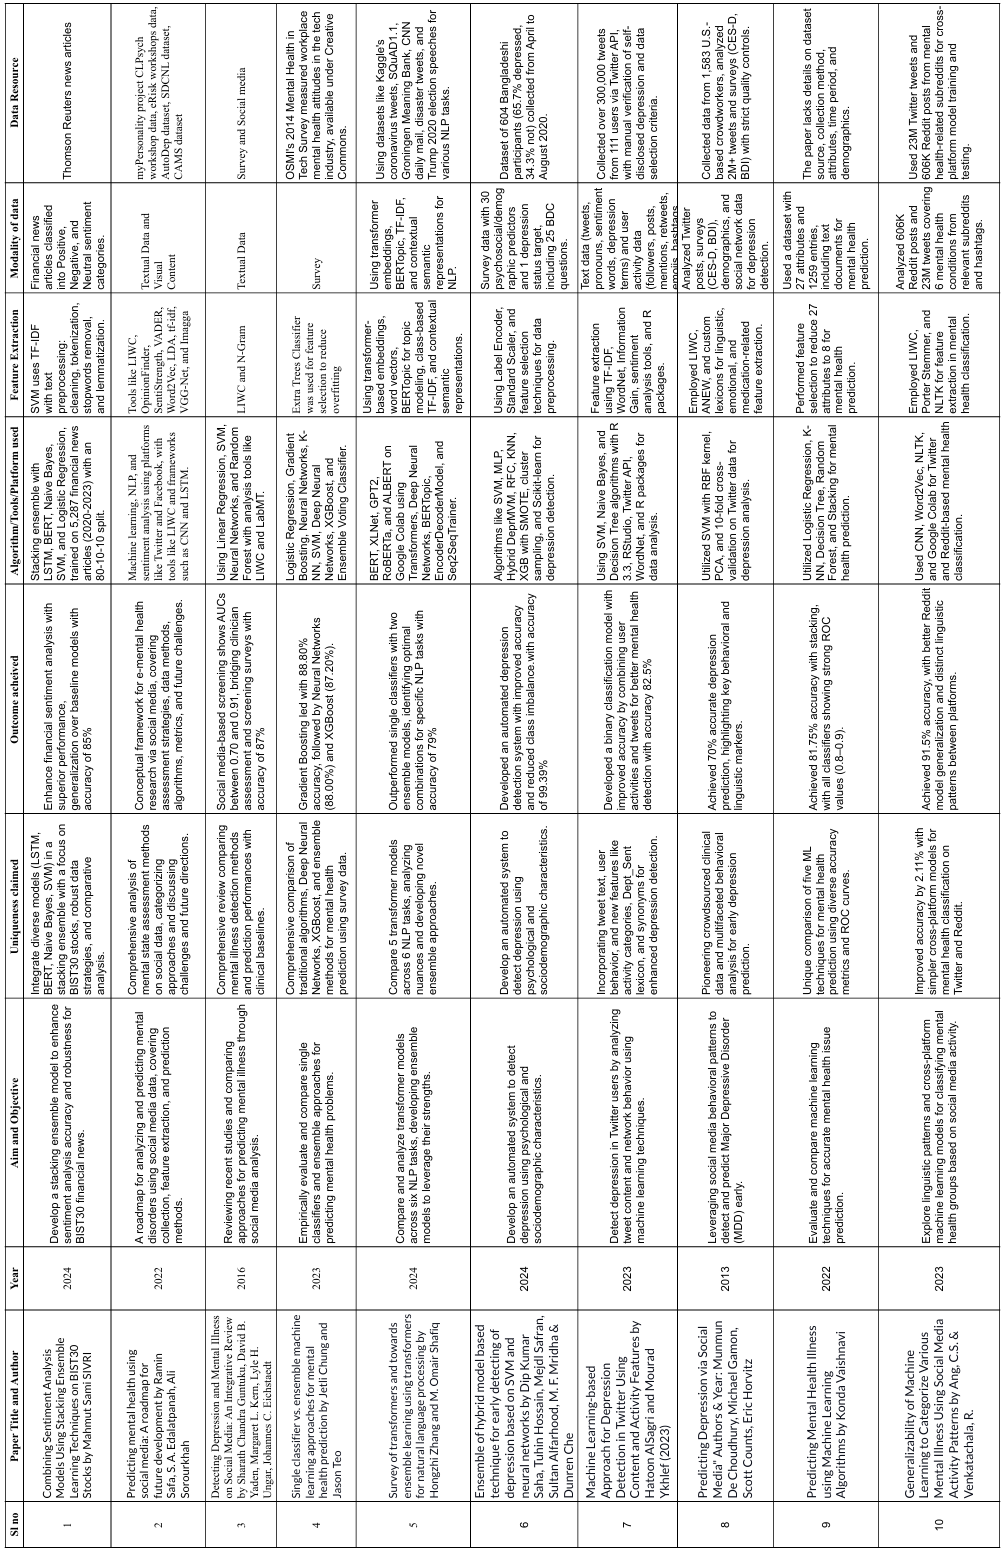
\includegraphics[width=0.89\textwidth]{Images/preframe-study.png}  
    \caption{Pre frame study review}
    \label{Preframe Study Review}  % Label for referencing the figure
\end{figure}


\pagebreak
% ----------------------------- Related Studies End --------------------------
